
Power dissipation is one of the critical factors for the development of wearable networks for high-end and low-end embedded devices. Therefore, a wide energy efficiency analysis, evaluating different factors in the design of the wearable devices, has great relevance. 
In a PSM, states are the modes of operation of the device. A transition between two states represents the energy cost and the delay spent consolidating state change. Thus, low power  states  have  a  longer  delay  between  transitions for states Run. The transition  time  is presented in~\cite{goraczko2008energy}, where it still infers that the times of the other transitions are insignificant and for the matter of simplicity not represented in the PSM.


Figure~\ref{fig:PSM_geral} represents the PSM of the wearable device we analyze in this work. %As we discussed in Section~\ref{sec:Methodology}, the wearable device presents three main states (idle, sleep and run). For the matter of simplicity, we have omitted in this figure transitions with negligible delays (e.g., Idle $\leftrightarrow$ Sleep). %According to this figure, 
Regardless the transmission mode on run state (i.e., ZigBee or Bluetooth), the sleep and idle states of the device present a mean energy consumption of 226.95\,mW and 236.21\,mW, respectively. The difference is of only 4.08\%, because wearable devices are automatically placed in low-power mode when they are not performing tasks. The sleep state presents a slightly higher transition time than the run state, when compared to the transition between the idle and run states. Thus, the fact that the idle state automatically operates at low power makes it attractive for exempting the developer from managing different sleep levels and their interruptions. 


\begin{figure}[tbh]
% \vspace{-0.3cm}
  \centering
  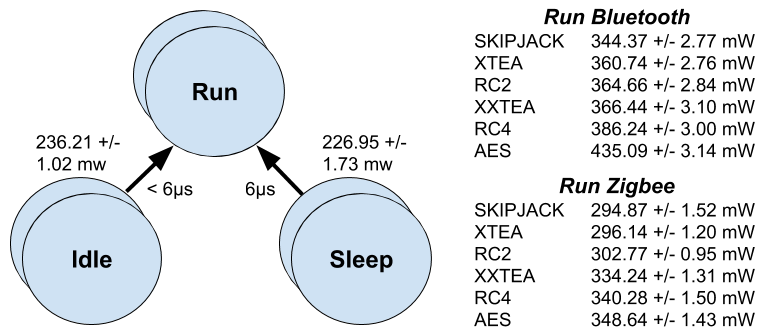
\includegraphics[scale=0.3]{Figures/C_PSM_geral.png}
  \caption{Wearable device power state machine (PSM)}
  \label{fig:PSM_geral}
 % \vspace{-0.3cm}
\end{figure}

\begin{figure*}[!t]
  %\vspace{-0.5cm}
\centering
  \begin{subfigure}[b]{0.4\textwidth}
    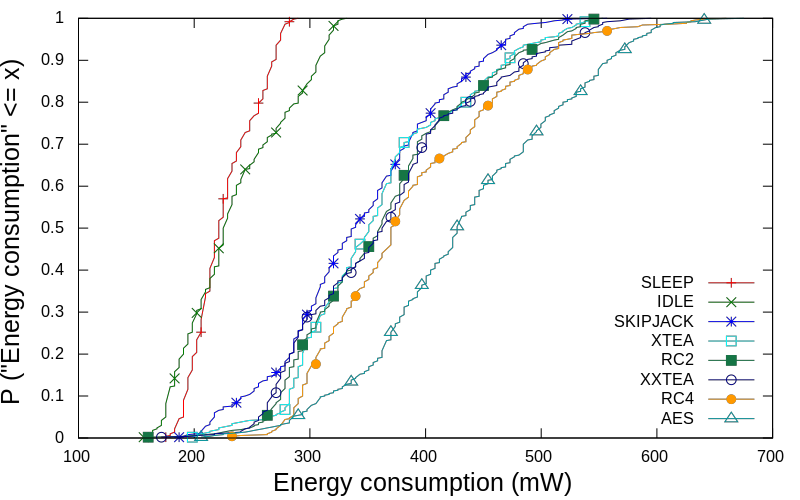
\includegraphics[width=\textwidth]{Figures/cdf_blue_aes.png}
    \caption{Power consumption per state using Bluetooth}
    \label{fig:cdf_blue}
  \end{subfigure}
  %
  \begin{subfigure}[b]{0.4\textwidth}
    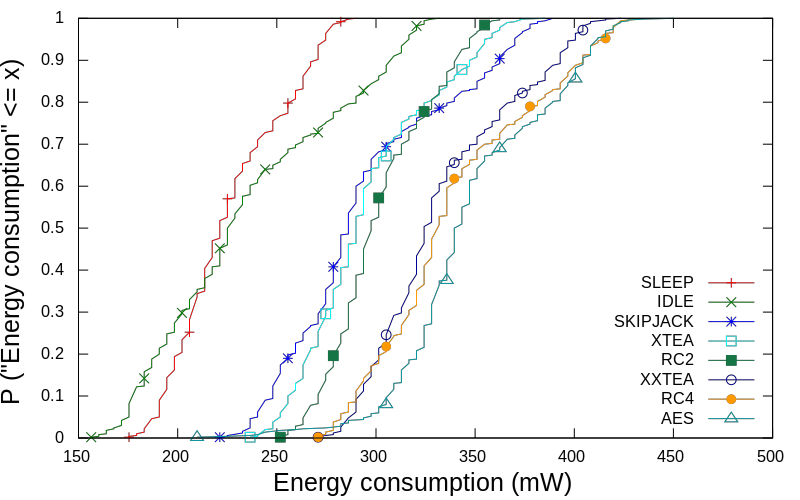
\includegraphics[width=\textwidth]{Figures/cdf_zig_aes.png}
    \caption{Power consumption per state using ZigBee}
    \label{fig:cdf_zig}
  \end{subfigure}
  \caption{Energy consumption on the run state}
  \vspace{-0.3cm}
\end{figure*}

Moreover, the run state, which encompasses data processing and transmission, asymptotically dominate energy consumption.  
For example, the run state using Bluetooth spends up to 71\% more energy, in the worst case, than the idle state. Clearly, for both transmission standards, SKIPJACK presents the lowest energy consumption among the evaluated algorithms. SKIPJACK, associated with Bluetooth or Zigbee, spends 12.16\% to 15.4\% less energy, respectively, than RC4 (which demands the highest amount of energy). Finally, ZigBee reduces the average energy consumption by 16.44\% when compared to Bluetooth.


%%%%%%%%%%%%%%%%%%%%%%%%%%%%%%%%%%%%%%%%%%%%%%%%%%%
\begin{comment}
\begin{table}[ht]
\centering
\caption{PSM Summary.}
%\vspace{0.3cm}
\label{table:papers}
\begin{tabular}{lccc}
\hline
\multicolumn{3}{c}{Transition latency}\\
\hline
Idle-Run & \multicolumn{2}{c}{$<$6us}\\
Sleep-Ru  & \multicolumn{2}{c}{6us}\\
\hline
\multicolumn{3}{c}{Energy Consumption}\\
\hline
Idle & \multicolumn{2}{c}{47.242}\\
Sleep & \multicolumn{2}{c}{45.390}\\
Run &  Bluetooth & Zigbee  \\
 \hline
SKIPJACK & 68.873 & 58.875 \\
XTEA  & 72.148 & 59.226 \\
RC2 & 72.931 & 60.554\\
XXTEA & 73.288 &  66.847\\
RC4 & 77.247 & 68.055
\end{tabular}
\end{table}

\end{comment}
%%%%%%%%%%%%%%%%%%%%%%%%%%%%%%%%%%%%%%%%%%%%%%%%%%

\begin{comment}
\begin{figure}[H]
 \vspace{-0.5cm}
  \centering
  \includegraphics[scale=0.25]{Figures/PSM_ZB.png}
  \caption{Power State Machine (PSM) using ZigBee.}
  \label{fig:PSM_ZB}
  %\vspace{-0.5cm}
\end{figure}
\end{comment}


%As Figuras~\ref{fig:cdf_blue} e~\ref{fig:cdf_zig} descrevem completamente a distribuição da probabilidade representado todos os cenários avaliados. A primeira referência a aplicação usando Bluetooth enquanto a segunda utiliza ZigBee. Deste modo, é possível notar que o comportamento do consumo dos métodos criptográficos ratificam os resultados apresentados pelo consumo médio. Com isto inferimos o Skipjack como método mais eficiente, opondo-se ao RC4, quando seu uso apresenta maior dissipação de energia.

Figures~\ref{fig:cdf_blue} and~\ref{fig:cdf_zig} %\abv{further 
detail the  energy consumption per state and  present the Cumulative Distribution Function (CDF) for each evaluated scenario. Figure~\ref{fig:cdf_blue} shows results when using Bluetooth, whereas Figure~\ref{fig:cdf_zig} presents results for the use of ZigBee. %It is possible to notice that 
Results for energy consumption following each cryptograph algorithm ratify the average energy consumption %\abv{
per state in Figure~\ref{fig:PSM_geral}. % and \ref{fig:PSM_ZB}. %  results presented by the average energy consumption. 
%Therefore, 
We observe SKIPJACK as the most efficient among all evaluated algorithms, and RC4 the least. % opposing RC4, when its use presents greater energy dissipation.

\begin{comment}
\begin{figure}[H]
  \centering
  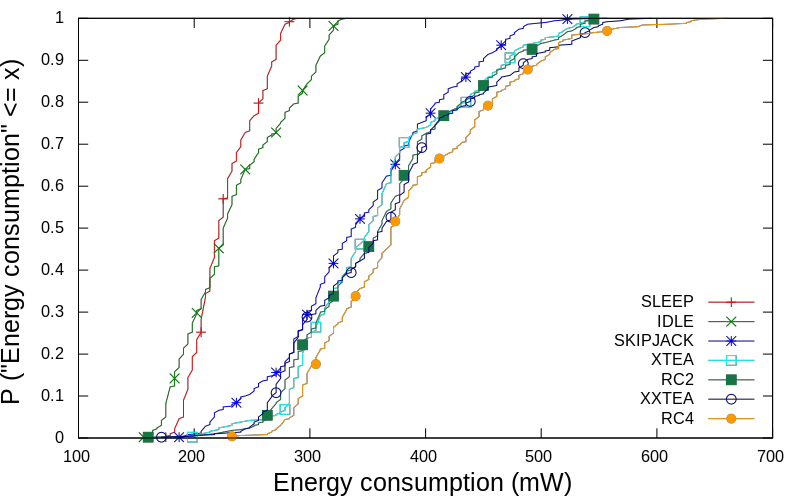
\includegraphics[scale=0.32]{Figures/cdf_blue_.png}
  \caption{Cumulative Distribution Function for energy consumption by state using Bluetooth.}
  \label{fig:cdf_blue}
\end{figure}

\begin{figure}[H]
  \centering
  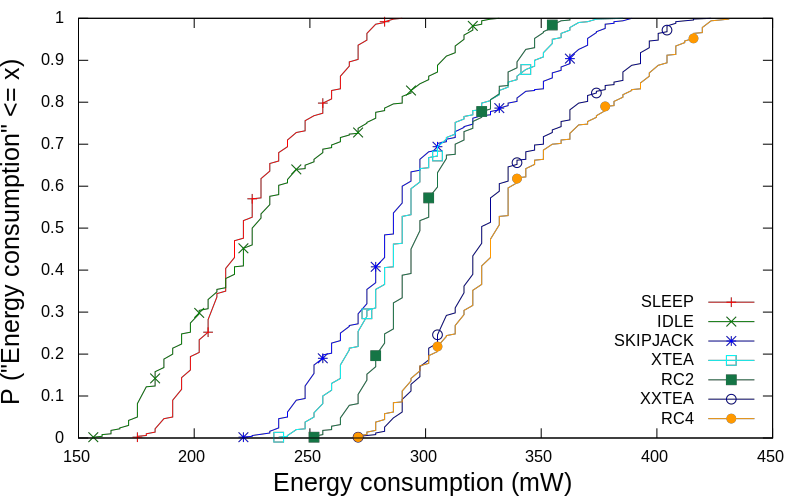
\includegraphics[scale=0.32]{Figures/cdf_zig_.png}
  \caption{Cumulative Distribution Function for energy consumption by state using ZigBee.}
  \label{fig:cdf_zig}
\end{figure}

\end{comment}



%%%%%%%%%%%%%%%%%%%%%%%%%%%%%%%%%%%%%%%%%%%%%%%%%%%%%%%%
%%%%%%%%%%%%% texto antigo    do inicio da seção %%%%%%%
%%%%%%%%%%%%%%%%%%%%%%%%%%%%%%%%%%%%%%%%%%%%%%%%%%%%%%%%
\begin{comment}
%A dissipação de energia é um dos fatores críticos para o desenvolvimento de sistemas para dispositivos embarcados de ponta e de baixo custo. Portanto uma análise de eficiência energética ampla, avaliando fatores distintos no projeto dos nós sensores possui grande relevância. Deste modo podemos representar os estados do nó com uma máquina de estado de potência (PSM), onde os estados são os modos de operação dos nós. As transições entre estados têm custo de energia e atraso. Assim, os modos de baixo consumo possuem maior atraso nas transições~\cite{benini2000survey}. Entretanto, algumas vezes este atraso pode ser insignificante.

Power dissipation is one of the critical factors for the development of wearable networks for high-end and low-end embedded devices. Therefore, a wide energy efficiency analysis, evaluating different factors in the design of the wearable devices, has great relevance. Hence, we represent the states of a given wearable device by a power state machine (PSM), where states are the modes of operation of the device. Transitions between states have energy cost and delay. Thus, low power modes have a longer delay in transitions~\cite{benini2000survey}, noting that sometimes this delay can be insignificant.

%Apoiando-se nisso, apresentamos um modelo abstrato simples do PSM para o nó sensor vestível e seus principais modos de atividade. O modo de processamento e a transmissão dos dados domina assintoticamente o consumo energético. Este, juntamente com os modos~\textit{idle} e~\textit{sleep}, representam os principais estados do nó na rede. Assim, a Figura~\ref{fig:PSM_BLUE} representa o PSM para o nó utilizando a transmissão de dados via Bluetooth. Por meio desta, podemos observar os estados com seus respectivos valores de dissipação de potência e as arestas de transição de estados e seus tempos. Este tempo referente às transições é apresentado em~\cite{goraczko2008energy}, onde ainda infere que os tempos das demais transições são insignificantes e por isso não representadas no PSM.


Figure~\ref{fig:PSM_geral} represents the PSM for \abv{a given wearable device} using Bluetooth for data transmission. We present a simple abstract model of PSM for a wearable device and its main states. Processing and data transmission modes asymptotically dominate energy consumption. This, along with the idle and sleep states, represents the major states of a wearable device in the network. In the figure, we observe the states with their respective values for power dissipation, state transitions and their times. Transition time follows~\cite{goraczko2008energy}, where it still infers that the times of the other transitions are insignificant and therefore not represented in the PSM, (e.g., Idle $\leftrightarrow$ Sleep).


\begin{figure}[tbh]
  \vspace{-0.3cm}
  \centering
  \includegraphics[scale=0.23]{Figures/PSM_blue.png}
  \caption{Power State Machine (PSM) using Bluetooth.}
  \label{fig:PSM_BLUE}
  \vspace{-0.2cm}
\end{figure}

%Observe que o modo~\textit{sleep} apresenta um menor consumo médio, 45.390 mA, contra 47.242 mA do modo~\textit{idle}. O que representa uma diferença de apenas 4,08\%. A estreita disparidade é justificada pelo fato do nó, automaticamente ser colocado em modo de baixa potência quando não está a executar tarefas. O modo~\textit{sleep} ainda apresenta tempo de transição levemente superior. Deste modo, o fato do modo~\textit{idle} operar em baixa potência automaticamente torna seu uso atraente. Isto pelo fato de isentar o desenvolvedor da função de gerenciar os diversos níveis de sono, bem como suas interrupções. Entre os algoritmos de criptografia a diferença no consumo médio chegou a 12.16\%. Destaque para o método SKIPJACK que se mostrou mais eficiente, em contraposição ao RC4.

%Note that 
Sleep mode has the lowest average energy consumption, 45,390 mA, compared to 47,242 mA in the idle mode. The difference is of % represents a difference  
only 4.08\%, because wearable devices are 
%
%The narrow difference is justified by the fact that the node is 
automatically placed in low power mode when they are not performing tasks. The sleep mode still has slightly higher transition time \abv{to running mode? falta um complemento na frase}. Thus, the fact that idle state automatically operates at low power makes it attractive for exempting the developer from managing different sleep levels and their interruptions. 
%
%. This is because it exempts the developer from the function of managing the various sleep levels, as well as their interruptions. 
Among the evaluated algorithms the difference of energy consumption, in average, reaches 12.16\%, highlighting SKIPJACK as the algorithm with the lowest energy consumption. %  more efficient, as opposed to RC4.

%De modo análogo, a Figura~\ref{fig:PSM_ZB}, proporciona a análise do consumo médio utilizando ZigBee como tecnologia de transmissão de dados. Deste modo, novamente destaca-se o método SKIPJACK como mais eficiente, dispondo de uma diferença de aproximadamente 15.4\% perante o método RC4. A partir destes dados podemos inferir também que optar por utilizar ZigBee como tecnologia de transmissão de dados proporciona uma eficiência energética média, na casa de 16.44\% em relação ao Bluetooth na média.

%Similarly, 
Figure~\ref{fig:PSM_ZB} provides the average energy consumption analysis when the wearable device uses ZigBee for data transmission. Again, SKIPJACK presents the lowest energy consumption, with a difference of approximately 15.4\% compared to RC4. We infer that ZigBee reduces the average energy consumption in 16.44\% compared to Bluetooth.

\end{comment}